\chapter{Visão Geral do Conjunto de Instruções}

\epigraph{``Por que os livros de matemática são tristes?
	Porque eles têm muitos problemas.''}


Este capítulo fornece uma visão geral básica de um subconjunto simples do conjunto de instruções x86-64 com foco nas operações inteiras. Isso abrangerá apenas o subconjunto de instruções necessárias para os tópicos e programas discutidos no escopo deste texto. Isso excluirá algumas das instruções mais avançadas e instruções de modo restrito. Para obter uma lista completa de todas as instruções do processador, consulte as referências listadas no Capítulo \ref{cap1}.

As instruções são apresentadas na seguinte ordem:
\begin{itemize}
	\item Movimentação de dados
	\item Instruções de conversão
	\item Instruções aritméticas
	\item Instruções lógicas
	\item Instruções de controle
\end{itemize}

As instruções para chamadas de funções são discutidas no capítulo no capítulo \ref{cap:Funções}, Funções.

Uma lista completa das instruções abordadas neste texto está localizada no Apêndice \ref{apendiceB} para referência.

\section{Convenções notacionais}
Esta seção resume a notação usada neste texto, que é bastante comum na literatura técnica. Em geral, uma instrução consiste na própria instrução ou operação (isto é, add, sub, mul, etc.) e nos \textbf{operandos}. Os operandos se referem de onde os dados (a serem operados) são provenientes e/ou onde o resultado deve ser colocado.

\subsection{Notação de Operando}
A Tabela \ref{tab:notacao} resume as convenções de notação usadas no restante do documento.

{\centering
	\begin{table}[ht]
		\centering
		\resizebox{0.8\textwidth}{!}{%
		\begin{tabular}{|p{3cm}|p{9cm}|}
			\hline
			\rowcolor[HTML]{C0C0C0} 
			{\color[HTML]{000000} } Notação de Operando & {\color[HTML]{000000} }Descrição \\ \hline
			\textbf{<reg>}& Operando registrador. O operando deve ser um registrador. \\ \hline
			\textbf{<reg8>,<reg16>, <reg32>,<reg64>} & Registrador operando com requisito de tamanho específico. Por exemplo, \textbf{reg8} significa apenas um registro de tamanho de byte (por exemplo, \textbf{al}, \textbf{bl}, etc.) e \textbf{reg32} significa um registro de tamanho de palavra dupla (por exemplo, \textbf{eax}, \textbf{ebx}, etc.).\\ \hline
			\textbf{<dest>} & Operando de destino. O operando pode ser um registro ou memória. Por ser um operando de destino, o conteúdo será sobrescrito pelo novo resultado (com base nas instruções específicas).\\ \hline
			\textbf{<RXdest>} & Operando de registro de destino de ponto flutuante. O operando deve ser um registrador de ponto flutuante. Por ser um operando de destino, o conteúdo será sobrescrito pelo novo resultado (com base nas instruções específicas).\\ \hline
			\textbf{<src>} & Operando de origem. O valor do operando é inalterado após a instrução.\\ \hline
			\textbf{<imm>} & Valor imediato. Pode ser especificado em decimal, hexadecimal, octal ou binário.\\ \hline
			\textbf{<mem>} & Localização da memória. Pode ser um nome de variável ou uma referência indireta (ou seja, um endereço de memória).\\ \hline
			\textbf{<op> ou <operand>} & Operando, registrador ou memória.\\ \hline
			\textbf{<op8>,<op16>, <op32>,<op64>} & Operando, registrador ou memória, com requisitos de tamanho específico. Por exemplo, \textbf{op8} significa apenas um operando de tamanho de byte e \textbf{reg32} significa apenas um operando de tamanho de palavra dupla.\\ \hline
			\textbf{<label>} & Rótulo do programa.\\ \hline
		\end{tabular}}
		\caption{Notação.}
		\label{tab:notacao}
	\end{table}
}

Por padrão, os valores imediatos são decimais ou base 10. Podem ser usados valores imediatos hexadecimais ou de base 16, mas devem ser precedidos por \textbf{0x} para indicar que o valor é hexadecimal. Por exemplo, $ 15_{10} $ pode ser inserido em hexadecimal como \textbf{0x0F}.

Consulte o Capítulo \ref{cap:ModosDeEndereçamento}, Modos de endereçamento para obter mais informações sobre os locais de memória e vias indiretas.

\section{Movimento de Dados}
Normalmente, os dados devem ser movidos para um registrador da CPU a partir da RAM para serem operados. Depois de concluídos os cálculos, o resultado pode ser copiado do registrador e colocado em uma variável. Existem várias fórmulas simples no programa de exemplo que executam essas etapas. Esta operação básica de movimentação de dados é realizada com a instrução de movimentação.

A forma geral da instrução de movimento é:\\
\textbf{mov <dest>, <src>}

O operando de origem (src) é copiado do operando de origem para o operando de destino. O valor do operando de origem permanece inalterado. O operando de destino e de origem devem ter o mesmo tamanho (ambos os bytes, ambas as palavras, etc.). O operando de destino não pode ser imediato. Ambos os operandos não podem ser memória. Se uma operação de memória para memória for necessária, duas instruções devem ser usadas.

\begin{figure}[h]
\begin{center}
		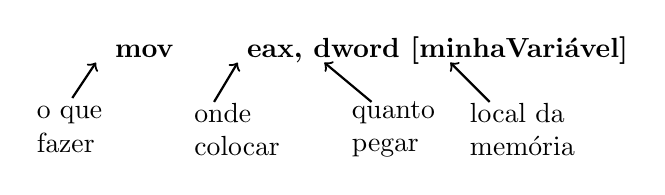
\begin{tikzpicture}
\node at (3.5cm,0) {\textbf{mov\hspace{0.8cm} eax, dword [minhaVariável]}};
\node at (0cm,-1cm) [text width=1.5cm] {o que fazer};
\node at (2cm,-1cm) [text width=1.5cm] {onde colocar};
\node at (4cm,-1cm) [text width=1.5cm] {quanto pegar};
\node at (5.5cm,-1cm) [text width=1.5cm] {local da memória};
\draw[thick,->] (-0.3cm,-0.6cm)--(0cm,-0.15cm);
\draw[thick,->] (1.5cm,-0.65cm)--(1.8cm,-0.15cm);
\draw[thick,->] (3.5cm,-0.65cm)--(2.9cm,-0.15cm);
\draw[thick,->] (5cm,-0.65cm)--(4.5cm,-0.15cm);
\end{tikzpicture}
\end{center}
	\caption{Visão geral instrução MOV.}
\end{figure}

Quando o operando do registrador de destino tem tamanho de palavra dupla e o operando de origem tem tamanho de palavra dupla, a palavra dupla de ordem superior do registrador de quatro palavras é definida como zero. Isso se aplica apenas quando o operando de destino é um registrador inteiro de palavra dupla.

Especificamente, se as seguintes operações forem realizadas,
\begin{verbatim}
mov 	eax, 100 	  ; eax = 0x00000064
mov 	rcx, -1  	  ; rcx = 0xffffffffffffffff
mov 	ecx, eax 	  ; ecx = 0x00000064
\end{verbatim}

Inicialmente, o registro \textbf{rcx} é definido como \textbf{-1} (que é todo \textbf{0xF}). Quando o número positivo do registrador \textbf{eax} ($ 100_{10}$) é movido para o registrador \textbf{rcx}, a parte de ordem superior do registrador \textbf{quadword rcx} é definida como \textbf{0} sobrescrevendo os 1s da instrução anterior.

A instrução de movimentação é resumida da seguinte forma:
\begin{table}[ht]
	\begin{center}
		%\resizebox{\textwidth}{!}{%
			\begin{tabular}{|ll|}
				\hline
				\rowcolor[HTML]{C0C0C0}
				\textbf{Instrução} & \textbf{Descrição} \\ 
				\textbf{mov <dest>, <fonte>} & Copie o operando de origem para o destino\\
				& operando.\\
				& \textit{Nota 1}, ambos os operandos não podem ser\\
				& memória.\\
				&Nota 2, operandos de destino não podem ser\\
				& imediatos.\\
				&Nota 3, para destino de palavra dupla e\\
				& operando de origem, a parte de ordem \\
				&superior do registrador de palavra \\
				&quádrupla é definida como 0. \\ \hline
		Exemplos:& \textbf{mov ax, 42}\\
		& \textbf{mov cl, byte [bvar]}\\
		& \textbf{mov dword [dVar], eax}\\
		& \textbf{mov qword [qVar], rdx}\\ \hline				
		\end{tabular}%}
	\end{center}
	\caption{Instrução MOV.}
	\label{tab:mov}
\end{table}

Uma lista mais completa das instruções está localizada no Apêndice \ref{apendiceB}.\\

Por exemplo, supondo as seguintes declarações de dados:
\begin{verbatim}
       dValue  dd    0
       bNum    db    42
       wNum    dw    5000
       dNum    dd    73000
       qNum    dq    73000000
       bAns    db    0
       wAns    dw    0
       dAns    dd    0
       qAns    dq    0
\end{verbatim}

Para realizar, as operações básicas de:
\begin{verbatim}
       dValue = 27
       bAns = bNum
       wAns = wNum
       dAns = dNum
       qAns = qNum
\end{verbatim}

As seguintes instruções podem ser usadas:
\begin{lstlisting}
mov dword [dValue], 27		; dValue = 27

mov al, byte [bNum]
mov byte [bAns], al 		; bAns = bNum

mov ax, word [wNum]
mov word [wAns], ax 		; wAns = wNum

mov eax, dword [dNum]
mov dword [dAns], eax 		; dAns = dNum

mov rax, qword [qNum]
mov qword [qAns], rax 		; qAns = qNum
\end{lstlisting}


Para algumas instruções, incluindo aquelas acima, a especificação de tipo explícita (por exemplo, byte, word, dword, qword) pode ser omitida, pois o outro operando definirá claramente o tamanho. No texto, ele será incluído por questões de consistência e boas práticas de programação.

\section{Endereços e Valores}
A única maneira de acessar a memória é com os colchetes ([]). A omissão dos colchetes não acessará a memória e, em vez disso, obterá o endereço do item. Por exemplo:
\begin{lstlisting}
mov rax, qword [var1]	; valor de var1 em rax
mov rax, var1           ; endereco de var1 em rax
\end{lstlisting}

Visto que omitir os colchetes não é um erro, o montador não gerará mensagens de erro ou avisos. Isso pode causar confusão.

Além disso, o endereço de uma variável pode ser obtido com o endereço efetivo de carga (\textit{load effective address}), ou instrução \textbf{lea}. A instrução de endereço efetivo de carga é resumida na Tabela \ref{tab:lea}:

\begin{table}[ht]
	\begin{center}
		%\resizebox{\textwidth}{!}
	\end{center}
	\caption{Instrução LEA.}
	\label{tab:lea}
\end{table}

Uma lista mais completa das instruções está localizada no Apêndice \ref{apendiceB}.

Informações adicionais e exemplos abrangentes são apresentados no Capítulo \ref{cap:ModosDeEndereçamento}, Modos de endereçamento.

\section{Instruções de conversão}
Às vezes, é necessário converter de um tamanho para outro. Por exemplo, um byte pode precisar ser convertido em uma palavra dupla para alguns cálculos em uma fórmula. O processo usado para conversões depende do tamanho e tipo do operando. As seções a seguir resumem como as conversões são realizadas.

\subsection{Conversões restritivas}
As conversões restritivas fazem a conversão de um tipo maior para um tipo menor (ou seja, palavra para byte ou palavra dupla para palavra).

Nenhuma instrução especial é necessária para conversões restritivas. A parte inferior da localização da memória ou registrador pode ser acessada diretamente. Por exemplo, se o valor de \textbf{50 (0x32)} for colocado no registrador \textbf{rax}, o registrador \textbf{al} pode ser acessado diretamente para obter o valor da seguinte forma:

\begin{lstlisting}
mov rax, 50
mov byte [bVal], al
\end{lstlisting}

Este exemplo é razoável, pois o valor de 50 caberá em um valor de byte. No entanto, se o valor de 500 (0x1f4) for colocado no registrador \textbf{rax}, o registrador \textbf{al} ainda pode ser acessado.
\begin{lstlisting}
mov rax, 500
mov byte [bVal], al
\end{lstlisting}

Neste exemplo, a variável \textbf{bVal} conterá \textbf{0xf4} que pode levar a resultados incorretos. O programador é responsável por garantir que as conversões de redução sejam realizadas de forma adequada. Ao contrário de um compilador, nenhum aviso ou mensagem de erro será gerado.

\subsection{Conversões expansivas}
As conversões de ampliação são de um tipo menor para um tipo maior (por exemplo, byte para palavra ou palavra para palavra dupla). Como o tamanho está sendo expandido, os bits de ordem superior devem ser definidos com base no sinal do valor original. Como tal, o tipo de dados, com ou sem sinal, deve ser conhecido e o processo ou instruções apropriados devem ser usados.

\subsubsection{Conversões sem sinal}
Para conversões de ampliação sem sinal, a parte superior da localização da memória ou registrador deve ser definida como zero. Como um valor sem sinal só pode ser positivo, os bits de ordem superior só podem ser zero. Por exemplo, para converter o valor de byte de 50 no registrador \textbf{al}, para um valor de quadword em \textbf{rbx}, as seguintes operações podem ser realizadas.
\begin{lstlisting}
mov al, 50
mov rbx, 0
mov bl, al
\end{lstlisting}

Como o registrador \textbf{rbx} foi definido como 0 e, em seguida, os 8 bits mais baixos foram definidos como o valor de \textbf{al} (50 neste exemplo), todo o registrador \textbf{rbx} de 64 bits agora é 50.

Este processo geral pode ser executado na memória ou em outros registradores. É responsabilidade do programador garantir que os valores sejam apropriados para os tamanhos de dados que estão sendo usados.

Uma conversão sem sinal de um tamanho menor para um tamanho maior também pode ser realizada com uma instrução de movimento especial, da seguinte maneira:
\begin{lstlisting}
movzx <dest>, <src>
\end{lstlisting}

Que preencherá os bits de ordem superior com zero. A instrução \textbf{movzx} não permite um operando de destino de palavra quádrupla com um operando de origem de palavra dupla. Como observado anteriormente, uma instrução \textbf{mov} com um operando de destino de registrador de palavra dupla com um operando de origem de palavra dupla zera a palavra dupla de ordem superior do registrador de destino de palavra dupla.

Um resumo das instruções que executam a conversão de alargamento sem sinal são as da Tabela \ref{tab:movzx}:

\begin{table}[ht]
	\begin{center}
		%\resizebox{\textwidth}{!}{%
		\begin{tabular}{|ll|}
			\hline
			\rowcolor[HTML]{C0C0C0}
			\textbf{Instrução} & \textbf{Descrição} \\ 
			\textbf{movzx <dest>, <src>} & Conversão com expansão sem sinal.\\
			\textbf{movzx <reg16>, <op8>} &\textit{Nota 1}, ambos os operandos não \\
			\textbf{movzx <reg32>, <op8>} &podem ser memória.\\
			\textbf{movzx <reg32>, <op16>} &\textit{Nota 2}, operandos de destino não \\
			\textbf{movzx <reg64>, <op8>} &podem ser imediatos.\\
			\textbf{movzx <reg64>, <op16>} &\textit{Nota 3}, valores imediatos não permitidos.\\ \hline
			Exemplos:& \textbf{movzx cx, byte [bVar]}\\
			& \textbf{movzx dx, al}\\
			& \textbf{movzx ebx, word [wVar]}\\
			& \textbf{movzx ebx, cx}\\
			& \textbf{movzx rbx, cl}\\
			& \textbf{movzx rbx, cx}\\ \hline				
		\end{tabular}%}
	\end{center}
	\caption{Instrução MOVZX.}
	\label{tab:movzx}
\end{table}

Uma lista mais completa das instruções está localizada no Apêndice \ref{apendiceB}.

\subsubsection{Conversões com sinal}
Para conversões com expansão com sinal, os bits de ordem superior devem ser definidos como 0 ou 1, dependendo se o valor original era positivo ou negativo.

Isso é executado por uma operação de extensão de sinal. Especificamente, o bit de ordem superior do valor original indica se o valor é positivo (com 0) ou negativo (com 1). O bit de ordem superior do valor original é estendido para os bits superiores do novo valor ampliado.

Por exemplo, dado que o registro ax está definido como \textbf{-7} (\textbf{0xfff9}), os bits seriam definidos da seguinte forma:

\begin{center}
	\resizebox{0.7\textwidth}{!}{%
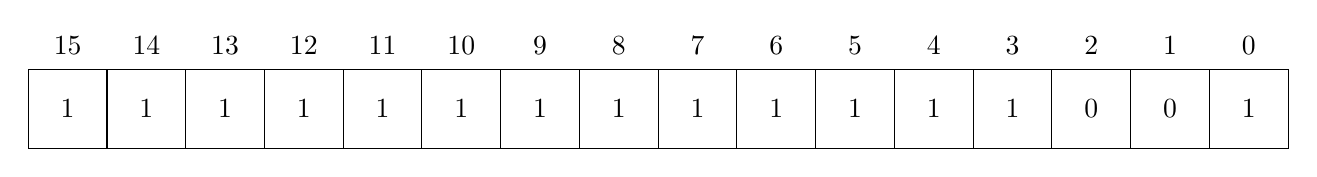
\begin{tikzpicture}

\foreach \x in {15,...,0}
  \draw (15-\x+0.5,1.3) node{\x};

\foreach \x in {0,1,2,...,16}
{
	
    \draw (\x,0) rectangle (1,1);
}
\foreach \x in {0,...,12}
   \draw (\x+0.5,0.5) node{1};
   
\draw (13.5,0.5) node{0};
\draw (14.5,0.5) node{0};
\draw (15.5,0.5) node{1};

\end{tikzpicture}
}
\end{center}

Como o valor é negativo, o bit de ordem superior (bit 15) é 1. Para converter o valor da palavra no registrador \textbf{ax} em um valor de palavra dupla no registrador \textbf{eax}, o bit de ordem superior (1 neste exemplo) é estendido ou copiado em toda a palavra de ordem superior (bits 31-16), resultando no seguinte:

\begin{center}
	\resizebox{\textwidth}{!}{%
		\begin{tikzpicture}
		
		\foreach \x in {31,...,0}
		\draw (31-\x+0.5,1.3) node{\x};
		
		\foreach \x in {0,1,2,...,32}
		{
			
			\draw (\x,0) rectangle (1,1);
		}
		\foreach \x in {0,...,28}
		\draw (\x+0.5,0.5) node{1};
		
		\draw (29.5,0.5) node{0};
		\draw (30.5,0.5) node{0};
		\draw (31.5,0.5) node{1};
		
		\end{tikzpicture}
	}
\end{center}

Há uma série de instruções dedicadas usadas para converter valores com sinal no registrador \textbf{A} de um tamanho menor para um tamanho maior. Essas instruções funcionam apenas no registrador \textbf{A}, às vezes usando o registrador \textbf{D} para o resultado. Por exemplo, a instrução \textbf{cwd} converterá um valor com sinal no registrador \textbf{ax} em um valor de palavra dupla nos registradores \textbf{dx} (parte de ordem superior) e \textbf{ax} (parte de ordem inferior). Normalmente, é por convenção escrito como \textbf{dx:ax}. A instrução \textbf{cwde} converterá um valor com sinal no registrador \textbf{ax} em um valor de palavra dupla no registrador \textbf{eax}.

Uma conversão com sinal mais generalizada de um tamanho menor para um tamanho maior também pode ser realizada com algumas instruções de movimento especiais, como segue:

\begin{lstlisting}
movsx <dest>, <src>
movsxd <dest>, <src>
\end{lstlisting}

Que executará a operação de extensão de sinal no argumento de origem. A instrução \textbf{movsx} é a forma geral e a instrução \textbf{movsxd} é usada para permitir um operando de destino de \textit{quadword} com um operando original de \textit{double-word}.

Um resumo das instruções que executam a conversão com expansão com sinal é apresentado nas Tabelas \ref{tab:cbw} e \ref{tab:movs}:

\begin{table}[ht]
	\begin{center}
		\resizebox{\textwidth}{!}{%
		\begin{tabular}{|ll|}
			\hline
			\rowcolor[HTML]{C0C0C0}
			\textbf{Instrução} & \textbf{Descrição} \\ 
			\textbf{cbw} & Converta \textit{byte} em \textbf{al} para \textit{word} em \textbf{ax}.\\
			& \textit{Nota}: só funciona em registrador \textbf{al} para \textbf{ax}.\\
			Exemplo:& \textbf{cbw}\\ \hline			
			\textbf{cwd} &Converta \textit{word} em \textbf{ax} para \textit{double word} em \textbf{dx:ax}.\\
			&\textit{Nota}: só funciona de \textbf{ax} para registradores \textbf{dx:ax}. \\
			Exemplo:& \textbf{cbd}\\ \hline			
			\textbf{cwde} &Converta \textit{word} em \textbf{ax} para \textit{double word} em \textbf{eax}.\\
			& \textit{Nota}: só funciona do registrador \textbf{ax} para \textbf{eax}.\\ 
			Exemplo:& \textbf{cwde}\\ \hline			
			\textbf{cdq} &Converta \textit{double word} em \textbf{eax} para \textit{quadword} em \textbf{edx:eax}.\\
			&\textit{Nota}: só funciona para do registrador \textbf{eax} para \textbf{edx:eax}. \\
			Exemplo:& \textbf{cdq}\\ \hline			
			\textbf{cdqe} &Converta \textit{double word} em \textbf{eax} para \textit{quadword} em \textbf{rax}.\\
			& \textit{Nota}: só funciona para registro rax.\\
			Exemplo:& \textbf{cdqe}\\ \hline			
			\textbf{cqo} &Converta \textit{quadword} em \textbf{rax} em \textit{double-quadword}\\
			& em \textbf{rdx:rax}.\\
			&\textit{Nota}: só funciona do registrador \textbf{rax} para \textbf{rdx:rax}.\\ 			
			Exemplo:& \textbf{cqo}\\ \hline
		\end{tabular}}
		\end{center}
	\caption{Instruções de expansão com sinal 1.}
\label{tab:cbw}
\end{table}
			
			
\begin{table}[ht]
	\begin{center}
		\resizebox{\textwidth}{!}{%
		\begin{tabular}{|ll|}
			\hline
			\rowcolor[HTML]{C0C0C0}
			\textbf{Instrução} & \textbf{Descrição} \\ 			
			\textbf{movsx <dest>, <src>} & Conversão de expansão com sinal\\
			& (via extensão de sinal).\\
			\textbf{movsx <reg16>, <op8>} &\textit{Nota 1}, ambos os operandos não \\
			\textbf{movsx <reg32>, <op8>} &podem ser memória.\\
			\textbf{movsx <reg32>, <op16>} &\textit{Nota 2}, operandos de destino não \\
			\textbf{movsx <reg64>, <op8>} &podem ser imediatos.\\
			\textbf{movsx <reg64>, <op16>} &\textit{Nota 3}, valores imediatos não permitidos.\\
			\textbf{movsxd <reg64>, <op32>}&\textit{Nota 4}: instrução especial (\textbf{movsxd}) necessária\\
			& para extensão assinada de 32 a 64 bits.\\ \hline
			Exemplos:& \textbf{movsx cx, byte [bVar]}\\
			& \textbf{movsx dx, al}\\
			& \textbf{movsx ebx, word [wVar]}\\
			& \textbf{movsx ebx, cx}\\
			& \textbf{movsxd rbx, dword [dVar]}\\\hline					
		\end{tabular}}
	\end{center}
	\caption{Instruções de expansão com sinal 2.}
	\label{tab:movs}
\end{table}

Uma lista mais completa das instruções está localizada no Apêndice \ref{apendiceB}.


\section{Instruções aritméticas inteiras}
As instruções aritméticas de inteiros realizam operações aritméticas como adição, subtração, multiplicação e divisão em valores inteiros. As seções a seguir apresentam as operações aritméticas básicas de inteiros.

\subsection{Adição}
A forma geral da instrução de adição de inteiro é a seguinte:\\
	\textbf{add	<dest>, <src>}

Onde a operação realiza o seguinte:\\
\textbf{<dest> = <dest> + <src>}

Especificamente, os operandos de origem e destino são adicionados e o resultado é colocado no operando de destino (sobrescrevendo o conteúdo anterior). O valor do operando de origem permanece inalterado. O operando de destino e de origem devem ter o mesmo tamanho (ambos os bytes, ambos words, etc.). O operando de destino não pode ser imediato. Ambos os operandos não podem ser memória. Se uma operação de adição de memória para memória for necessária, duas instruções devem ser usadas.

Por exemplo, supondo as seguintes declarações de dados:
\begin{lstlisting}
bNum1   db 42
bNum2   db 73
bAns    db 0

wNum1   dw   4321
wNum2   dw   1234
wAns    dw   0

dNum1   dd 42000
dNum2   dd 73000
dAns    dd 0

qNum1   dq 42000000
qNum2   dq 73000000
qAns    dq 0
\end{lstlisting}

Para realizar as operações básicas de:

\begin{tabular}{rlcl}
	\textbf{bAns} & = \textbf{bNum1} &\textbf{+}& \textbf{bNum2}\\
	\textbf{wAns} & = \textbf{wNum1} &\textbf{+}& \textbf{wNum2}\\
	\textbf{dAns} & = \textbf{dNum1} &\textbf{+}& \textbf{dNum2}\\
	\textbf{qAns} & = \textbf{qNum1} &\textbf{+}& \textbf{qNum2}\\
\end{tabular}

As seguintes instruções podem ser usadas:
\begin{lstlisting}
; bAns = bNum1 + bNum2
mov al, byte [bNum1]
add al, byte [bNum2]
mov byte [bAns], al

; wAns = wNum1 + wNum2
mov ax, word [wNum1]
add ax, word [wNum2]
mov word [wAns], ax

; dAns = dNum1 + dNum2
mov eax, dword [dNum1]
add eax, dword [dNum2]
mov dword [dAns], eax

; qAns = qNum1 + qNum2
mov rax, qword [qNum1]
add rax, qword [qNum2]
mov qword [qAns], rax
\end{lstlisting}

Para algumas instruções, incluindo aquelas acima, a especificação explícita de tipo  (por exemplo, byte, word, dword, qword) pode ser omitida, pois o outro operando definirá claramente o tamanho. Ele está incluído para consistência e boas práticas de programação.

Além da instrução \textbf{add} básica, há uma instrução de incremento que adicionará um ao operando especificado. A forma geral da instrução de incremento é a seguinte:\\
\textbf{inc <operando>}\\
Na qual a operação é a seguinte:\\
\textbf{<operando> = <operando> + 1}

O resultado é exatamente o mesmo que usar a instrução \textbf{add} (e adicionar um). Ao usar um operando de memória, a especificação de tipo explícita (por exemplo, \textit{byte}, \textit{word}, \textit{dword}, \textit{qword}) é necessária para definir claramente o tamanho.

Por exemplo, supondo as seguintes declarações de dados:
\begin{lstlisting}
bNum db 42
wNum dw 4321
dNum dd 42000
qNum dq 42000000
\end{lstlisting}

Para realizar, as operações básicas de:\\
\textbf{rax = rax + 1\\
bNum = bNum + 1\\
wNum = wNum + 1\\
dNum = dNum + 1\\
qNum = qNum + 1\\}

As seguintes instruções podem ser usadas:
\begin{lstlisting}
inc rax           ; rax = rax + 1
inc byte [bNum]   ; bNum = bNum + 1
inc word [wNum]   ; wNum = wNum + 1
inc dword [dNum]  ; dNum = dNum + 1
inc qword [qNum]  ; qNum = qNum + 1
\end{lstlisting}

A instrução de adição opera da mesma forma em dados com e sem sinal. É responsabilidade do programador garantir que os tipos e tamanhos de dados sejam apropriados para as operações realizadas.

As instruções de adição de inteiros são resumidas na Tabela \ref{tab:add}:

\begin{table}[ht]
	\begin{center}
		%\resizebox{\textwidth}{!}{%
			\begin{tabular}{|ll|}
				\hline
				\rowcolor[HTML]{C0C0C0}
				\textbf{Instrução} & \textbf{Descrição} \\ 
				\textbf{add <dest>, <src>} & Adicione dois operandos, (\textbf{<dest>} + \textbf{<src>})\\
				& e coloque o resultado em \textbf{<dest>}\\
				&(sobrescrevendo o valor anterior).\\
				& \textit{Nota 1}: ambos os operandos não podem ser memória.\\
				& \textit{Nota 2}: o operando de destino não pode ser imediato.\\
			   Exemplos:& add cx, word [wVvar]\\
			   &add rax, 42\\
			   &add dword [dVar], eax\\
			   &add qword [qVar], 300\\\hline
			   \textbf{inc <operando>} &Incremente <operando> em 1.\\
			   Exemplos:& inc word [wVvar]\\
			   &inc rax\\
			   &inc dword [dVar]\\
			   &inc qword [qVar]\\ \hline			   	
		\end{tabular}%}
	\end{center}
	\caption{Instruções de adição.}
	\label{tab:add}
\end{table}

Uma lista mais completa das instruções está localizada no Apêndice \ref{apendiceB}.

\subsubsection{Adição com Carry}
A adição com transporte é uma instrução especial de adição que incluirá um transporte de uma operação de adição anterior. Isso é útil ao adicionar números muito grandes, especificamente números maiores que o tamanho do registro da máquina.

Usar um carry adicional é bastante normal. Por exemplo, considere a seguinte operação.

\begin{center}
	
		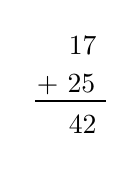
\begin{tikzpicture}
\node at (0,0) {17};	
\node at (-0.21,-0.5) {+ 25};
\draw [thick] (-0.6,-0.7) -- (0.3,-0.7);
\node at (0,-1) {42};	
		\end{tikzpicture}
\end{center}

Como você deve se lembrar, os dígitos menos significativos (7 e 5) são adicionados primeiro. O resultado de 12 é anotado como 2 com 1 de transporte (\textit{carry}). Os dígitos mais significativos (1 e 2) são adicionados junto com o transporte anterior (1 neste exemplo) resultando em 4.

Como tal, são necessárias duas operações de adição. Como não há transporte possível com a parte menos significativa, uma instrução de adição regular é usada. A segunda operação de adição precisaria incluir um possível transporte da operação anterior e deve ser feita com uma adição com instrução de transporte. Além disso, a adição com carry deve seguir imediatamente a operação de adição inicial para garantir que o registrador \textbf{rFlag} não seja alterado por uma instrução não relacionada (portanto, possivelmente alterando o bit de transporte).

Para programas em linguagem \textit{assembly}, a \textit{quadword} Menos Significativa (LSQ, do inglês \textit{Least Significant Quadword}) é adicionada com a instrução \textbf{add} e, em seguida, imediatamente a \textit{quadword} mais significativa (MSQ, do inglês \textit{Most Significant Quadword}) é adicionada com o \textbf{adc}, que adicionará as quadwords e incluirá um transporte da operação de adição anterior.

A forma geral da instrução de adição inteira  com transporte é a seguinte:
\begin{center}
	\textbf{adc <dest>, <src>}
\end{center}

Na qual a operação realiza o seguinte:
\begin{center}
	\textbf{<dest> = <dest> + <src> + <carryBit>}
\end{center}

Especificamente, os operandos de origem e destino junto com o bit de transporte são adicionados e o resultado é colocado no operando de destino (sobrescrevendo o valor anterior). O carry é parte do registrador \textbf{rFlag}. O valor do operando de origem permanece inalterado. O operando de destino e de origem devem ter o mesmo tamanho (ambos os bytes, ambas as words, etc.). O operando de destino não pode ser imediato. Ambos os operandos não podem ser memória. Se uma operação de adição de memória para memória for necessária, duas instruções devem ser usadas.

Por exemplo, dadas as seguintes declarações;
\begin{lstlisting}
dquad1 ddq 0x1A000000000000000
dquad2 ddq 0x2C000000000000000
dqSum  ddq 0
\end{lstlisting}

Cada uma das variáveis \textbf{\textit{dquad1}}, \textbf{\textit{dquad2}} e \textbf{\textit{dqSum}} tem 128 bits e, portanto, excederá o tamanho do registro de 64 bits da máquina. No entanto, dois registradores de 64 bits podem ser usados para cada um dos valores de 128 bits. Isso requer duas instruções de movimentação, uma para cada registrador de 64 bits. Por exemplo,

\begin{lstlisting}
mov rax, qword [dquad1]
mov rdx, qword [dquad1+8]
\end{lstlisting}

O primeiro movimento para o registrador \textbf{rax} acessa os primeiros 64 bits da variável de 128 bits. O segundo movimento para o registro \textbf{rdx} acessa os próximos 64 bits da variável de 128 bits. Isso é feito usando o endereço inicial da variável, \textit{\textbf{dquad1}}, e adicionando 8 bytes, pulando assim os primeiros 64 bits (ou 8 bytes) e acessando os próximos 64 bits.

Se os \textit{LSQs} forem adicionados e, em seguida, os \textit{MSQs} forem adicionados incluindo qualquer transporte, o resultado de 128 bits pode ser obtido corretamente. Por exemplo,
\begin{lstlisting}
mov rax, qword [dquad1]
mov rdx, qword [dquad1+8]

add rax, qword [dquad2]
adc rdx, qword [dquad2+8]

mov qword [dqSum], rax
mov qword [dqSum+8], rdx
\end{lstlisting}


Inicialmente, o \textit{LSQ} de \textbf{dquad1} é colocado em \textbf{rax} e o \textit{MSQ} é colocado em \textbf{rdx}. Em seguida, a instrução \textbf{add} adicionará o \textbf{rax} de 64 bits com o \textit{LSQ} de \textbf{dquad2} e, neste exemplo, fornecerá um transporte de 1 com o resultado em \textbf{rax}. Em seguida, o \textbf{rdx} é adicionado com o \textit{MSQ} de \textbf{dquad2} junto com o transporte por meio da instrução \textbf{adc} e o resultado colocado em \textbf{rdx}.

A adição de inteiro com instrução de transporte é resumida da seguinte forma:

\begin{table}[ht]
	\begin{center}
		\resizebox{\textwidth}{!}{%
		\begin{tabular}{|ll|}
			\hline
			\rowcolor[HTML]{C0C0C0}
			\textbf{Instrução} & \textbf{Descrição} \\ 
			\textbf{adc <dest>, <src>} & Adicione dois operandos, (<dest> + <src>) e\\
			&qualquer carry anterior (armazenado no bit de\\
			& transporte no registrador rFlag) \\
			& e coloque o resultado em \textbf{<dest>}\\
			&(sobrescrevendo o valor anterior).\\
			& \textit{Nota 1}: ambos os operandos não podem ser memória.\\
			& \textit{Nota 2}: o operando de destino não pode ser imediato.\\
			Exemplos:& \textbf{adc rcx, qword [dVvar]}\\
			&\textbf{adc rax, 4}2\\ \hline			   	
		\end{tabular}}
	\end{center}
	\caption{Instruções de adição.}
	\label{tab:adc}
\end{table}

Uma lista mais completa das instruções está localizada no Apêndice \ref{apendiceB}.

\subsection{Subtraction}

A forma geral da instrução de subtração de inteiro é a seguinte:
\begin{center}
	\textbf{sub <dest>, <src>}
\end{center}

Na qual a operação realiza o seguinte:
\begin{center}
	\textbf{<dest> = <dest> - <src>}
\end{center}

Especificamente, o operando de origem é subtraído do operando de destino e o resultado é colocado no operando de destino (sobrescrevendo o valor anterior). O valor do operando de origem permanece inalterado. O operando de destino e de origem devem ter o mesmo tamanho (ambos os bytes, ambas as words, etc.). O operando de destino não pode ser imediato. Ambos os operandos não podem ser memória. Se uma operação de subtração de memória para memória for necessária, duas instruções devem ser usadas.

Por exemplo, supondo as seguintes declarações de dados:
\begin{lstlisting}
bNum1   db 73
bNum2   db 42
bAns    db 0

wNum1   dw   1234
wNum2   dw   4321
wAns    dw   0

dNum1   dd 73000
dNum2   dd 42000
dAns    dd 0

qNum1   dq 73000000
qNum2   dq 42000000
qAns    dq 0
\end{lstlisting}

Para realizar, as operações básicas de:\\
\begin{tabular}{rlcl}
	\textbf{bAns} & = \textbf{bNum1} &\textbf{-}& \textbf{bNum2}\\
	\textbf{wAns} & = \textbf{wNum1} &\textbf{-}& \textbf{wNum2}\\
	\textbf{dAns} & = \textbf{dNum1} &\textbf{-}& \textbf{dNum2}\\
	\textbf{qAns} & = \textbf{qNum1} &\textbf{-}& \textbf{qNum2}\\
\end{tabular}

As seguintes instruções podem ser usadas:
\begin{lstlisting}
; bAns = bNum1 - bNum2
mov al, byte [bNum1]
sub al, byte [bNum2]
mov byte [bAns], al

; wAns = wNum1 - wNum2
mov ax, word [wNum1]
sub ax, word [wNum2]
mov word [wAns], ax

; dAns = dNum1 - dNum2
mov eax, dword [dNum1]
sub eax, dword [dNum2]
mov dword [dAns], eax

; qAns = qNum1 - qNum2
mov rax, qword [qNum1]
sub rax, qword [qNum2]
mov qword [qAns], rax
\end{lstlisting}

Para algumas instruções, incluindo aquelas acima, a especificação explícita de tipo  (por exemplo, \textit{byte}, \textit{word}, \textit{dword}, \textit{qword}) pode ser omitida, pois o outro operando definirá claramente o tamanho. Ele está incluído para consistência e boas práticas de programação.

Além da instrução de subtração básica, há uma instrução de decremento que subtrairá um do operando especificado. A forma geral da instrução de decremento é a seguinte:
\textbf{dec <operando>}\\
Na qual a operação é a seguinte:\\
\textbf{<operando> = <operando> - 1}

O resultado é exatamente o mesmo que usar a instrução \textbf{sub} (e subtrair um). Ao usar um operando de memória, a especificação de tipo explícita (por exemplo, \textit{byte}, \textit{word}, \textit{dword}, \textit{qword}) é necessária para definir claramente o tamanho.

Por exemplo, supondo as seguintes declarações de dados:
\begin{lstlisting}
bNum db 42
wNum dw 4321
dNum dd 42000
qNum dq 42000000
\end{lstlisting}

Para realizar, as operações básicas de:\\
\textbf{rax = rax - 1\\
	bNum = bNum - 1\\
	wNum = wNum - 1\\
	dNum = dNum - 1\\
	qNum = qNum - 1\\}

As seguintes instruções podem ser usadas:
\begin{lstlisting}
dec rax           ; rax = rax - 1
dec byte [bNum]   ; bNum = bNum - 1
dec word [wNum]   ; wNum = wNum - 1
dec dword [dNum]  ; dNum = dNum - 1
dec qword [qNum]  ; qNum = qNum - 1
\end{lstlisting}

A instrução de subtração opera da mesma forma em dados com e sem sinal. É responsabilidade do programador garantir que os tipos e tamanhos de dados sejam apropriados para as operações realizadas.

As instruções de subtração de inteiros são resumidas na Tabela \ref{tab:add}:

\begin{table}[ht]
	\begin{center}
		%\resizebox{\textwidth}{!}{%
		\begin{tabular}{|ll|}
			\hline
			\rowcolor[HTML]{C0C0C0}
			\textbf{Instrução} & \textbf{Descrição} \\ 
			\textbf{sub <dest>, <src>} & Subtraia dois operandos, (\textbf{<dest>} - \textbf{<src>})\\
			& e coloque o resultado em \textbf{<dest>}\\
			&(sobrescrevendo o valor anterior).\\
			& \textit{Nota 1}: ambos os operandos não podem ser memória.\\
			& \textit{Nota 2}: o operando de destino não pode ser imediato.\\
			Exemplos:& sub cx, word [wVvar]\\
			&sub rax, 42\\
			&sub dword [dVar], eax\\
			&sub qword [qVar], 300\\\hline
			\textbf{dec <operando>} &Decremente <operando> de 1.\\
			Exemplos:& dec word [wVvar]\\
			&dec rax\\
			&dec dword [dVar]\\
			&dec qword [qVar]\\ \hline			   	
		\end{tabular}%}
	\end{center}
	\caption{Instruções de subtração.}
	\label{tab:sub}
\end{table}

Uma lista mais completa das instruções está localizada no Apêndice \ref{apendiceB}.

\subsection{Multiplicação Inteira}
A instrução de multiplicação multiplica dois operandos inteiros. Matematicamente, existem regras especiais para lidar com a multiplicação de valores com sinais. Como tal, instruções diferentes são usadas para multiplicação sem sinal (\textbf{mul}) e multiplicação com sinal (\textbf{imul}).

A multiplicação normalmente produz resultados de tamanho duplo. Ou seja, a multiplicação de dois valores de \textit{n} bits produz um resultado de \textit{2n} bits. Multiplicar dois números de 8 bits produzirá um resultado de 16 bits. Da mesma forma, a multiplicação de dois números de 16 bits produzirá um resultado de 32 bits, a multiplicação de dois números de 32 bits produzirá um resultado de 64 bits e a multiplicação de dois números de 64 bits produzirá um resultado de 128 bits.

Existem muitas variantes para a instrução de multiplicação. Para a multiplicação com sinal, algumas formas truncarão o resultado para o tamanho dos operandos originais. É responsabilidade do programador garantir que os valores usados funcionarão para as instruções específicas selecionadas.

\subsubsection{Multiplicação sem sinal}
A forma geral da multiplicação sem sinal é a seguinte:
\begin{center}
	\textbf{mul <src>}
\end{center}

Na qual o operando de origem deve ser um registrador ou local de memória. Um operando imediato não é permitido.

Para a instrução de multiplicação de operando único, o registraor \textbf{A} (\textbf{al}/\textbf{ax}/\textbf{eax}/\textbf{rax}) deve ser usado para um dos operandos (\textbf{al} para 8 bits, \textbf{ax} para 16 bits, \textbf{eax} para 32 bits e \textbf{rax} para 64 -mordeu). O outro operando pode ser um local ou registro da memória, mas não imediato. Além disso, o resultado será colocado nos registros \textbf{A} e possivelmente \textbf{D}, com base nos tamanhos que estão sendo multiplicados. A Figura \ref{fig:multiplica} mostra as várias opções para multiplicações sem sinal de \textbf{byte}, \textbf{word}, \textbf{double-word} e \textbf{quad-word}.

\begin{figure}[ht]
\begin{center}
		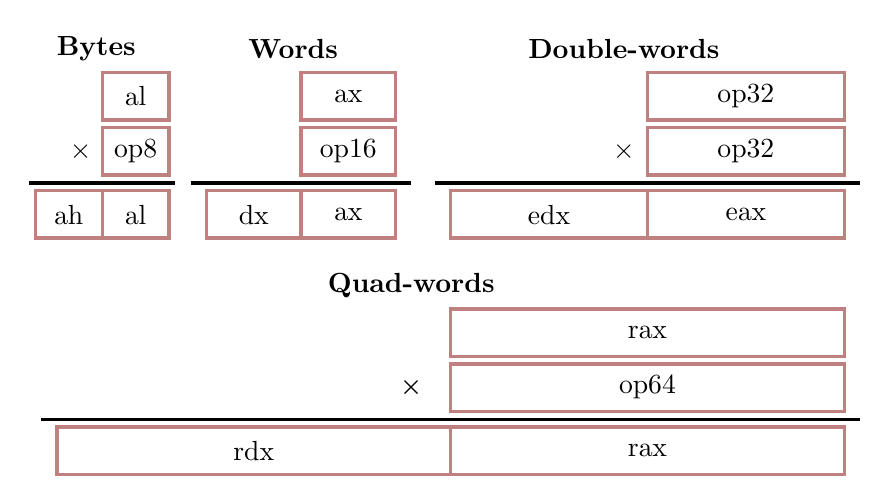
\begin{tikzpicture}
\node [very thick, draw=red!50!black!50, minimum width=5cm, minimum height=0.6cm] at (0,0) {rdx};
\node [very thick, draw=red!50!black!50, minimum width=5cm, minimum height=0.6cm] at (5,0) {rax};

\draw[very thick] (-2.7,0.4)--(7.7,0.4);

\node [very thick, draw=red!50!black!50, minimum width=5cm, minimum height=0.6cm] at (5,0.8) {op64};
\node at (2,0.8) {$\times$};
\node [very thick, draw=red!50!black!50, minimum width=5cm, minimum height=0.6cm] at (5,1.5) {rax};

\node at (2,2.1) {\textbf{Quad-words}};
\node at (4.7,5.1) {\textbf{Double-words}};
\node at (0.5,5.1) {\textbf{Words}};
\node at (-2,5.1) {\textbf{Bytes}};

\node [very thick, draw=red!50!black!50, minimum width=0.85cm, minimum height=0.6cm] at (-2.35,3) {ah};
\node [very thick, draw=red!50!black!50, minimum width=0.85cm, minimum height=0.6cm] at (-1.5,3) {al};
\draw[very thick] (-2.85,3.4)--(-1,3.4);
\node [very thick, draw=red!50!black!50, minimum width=0.85cm, minimum height=0.6cm] at (-1.5,3.8) {op8};
\node at (-2.2,3.8) {$\times$};
\node [very thick, draw=red!50!black!50, minimum width=0.85cm, minimum height=0.6cm] at (-1.5,4.5) {al};

\node [very thick, draw=red!50!black!50, minimum width=2.5cm, minimum height=0.6cm] at (3.75,3) {edx};
\node at (2,0.8) {$\times$};
\node [very thick, draw=red!50!black!50, minimum width=2.5cm, minimum height=0.6cm] at (6.25,3) {eax};
\draw[very thick] (2.3,3.4)--(7.7,3.4);

\node [very thick, draw=red!50!black!50, minimum width=1.2cm, minimum height=0.6cm] at (0,3) {dx};
\node [very thick, draw=red!50!black!50, minimum width=1.2cm, minimum height=0.6cm] at (1.2,3) {ax};
\draw[very thick] (-0.8,3.4)--(2,3.4);
\node [very thick, draw=red!50!black!50, minimum width=1.2cm, minimum height=0.6cm] at (1.2,3.8) {op16};
\node [very thick, draw=red!50!black!50, minimum width=1.2cm, minimum height=0.6cm] at (1.2,4.5) {ax};

\node [very thick, draw=red!50!black!50, minimum width=2.5cm, minimum height=0.6cm] at (6.25,3.8) {op32};
\node at (4.7,3.8) {$\times$};
\node [very thick, draw=red!50!black!50, minimum width=2.5cm, minimum height=0.6cm] at (6.25,4.5) {op32};

\end{tikzpicture}
\end{center}
	\caption{Visão geral da multiplicação de inteiros }
	\label{fig:multiplica}
\end{figure}

Conforme mostrado no gráfico, na maioria dos casos, a multiplicação inteira usa uma combinação dos registradores A e D. Isso pode ser muito confuso.

Por exemplo, ao multiplicar um \textbf{rax} (64 bits) vezes um operando de palavra quádrupla (64 bits), a instrução de multiplicação fornece um resultado de dupla palavra quádrupla  (128 bits). Isso pode ser útil e importante ao lidar com números muito grandes. Uma vez que a arquitetura de 64 bits tem apenas registros de 64 bits, o resultado de 128 bits é, e deve ser, colocado em dois registros de palavras quádruplas (64 bits) diferentes, \textbf{rdx} para o resultado de ordem superior e \textbf{rax} para o resultado de ordem inferior, que normalmente é escrito como \textbf{rdx:rax} (por convenção).

No entanto, esse uso de dois registradores também se aplica a tamanhos menores. Por exemplo, o resultado da multiplicação de \textbf{ax} (16 bits) vezes um operando de \textit{word} (também 16 bits) fornece um resultado de palavra dupla (32 bits). No entanto, o resultado não é colocado em \textbf{eax} (o que pode ser mais fácil), ele é colocado em dois registradores, \textbf{dx} para o resultado de ordem superior (16 bits) e \textbf{ax} para o resultado de ordem inferior (16 bits), normalmente escrito como \textbf{dx:ax} (por convenção). Como o resultado de palavra dupla (32 bits) está em dois registradores diferentes, podem ser necessários dois movimentos para salvar o resultado.

Esse par de registradores, mesmo quando não obrigatório, é devido ao suporte legado para versões anteriores da arquitetura. Embora isso ajude a garantir a compatibilidade com versões anteriores, pode ser bastante confuso.

Por exemplo, supondo as seguintes declarações de dados:
\begin{lstlisting}
bNumA   db 42
bNumB   db 73
wAns    db 0
wAns1   db 0

wNumA   dw   4321
wNumB   dw   1234
dAns2   dw   0

dNumA   dd 42000
dNumB   dd 73000
dAns3   dd 0

qNumA   dq 420000
qNumB   dq 730000
dqAns4  dq 0
\end{lstlisting}

Para realizar, as operações básicas de:\\
\begin{tabular}{llcl}
	\textbf{wAns} & = \textbf{bNumA\^{}2} &&; quadrado de bNumA\\
	\textbf{wAns1} & = \textbf{bNumA} &\textbf{*}& \textbf{bNumB}\\
	\textbf{dAns2} & = \textbf{wNumA} &\textbf{*}& \textbf{wNumB}\\
	\textbf{qAns3} & = \textbf{dNumA} &\textbf{*}& \textbf{dNumB}\\
	\textbf{dqAns4} & = \textbf{qNumA} &\textbf{*}& \textbf{qNumB}\\
\end{tabular}

As seguintes instruções podem ser usadas:
\begin{lstlisting}
; wAns = bNumA^2 ou bNumA ao quadrado
mov al, byte [bNumA]
mul al                  ; resultado em ax
mov word [wAns], ax

; wAns1 = bNumA * bNumB
mov al, byte [bNumA]
mul byte [bNumB]        ; resultado em ax
mov word [wAns1], ax

; dAns2 = wNumA * wNumB
mov ax, word [wNumA]
mul word [wNumB]        ; resultado em dx:ax
mov word [dAns2], ax
mov word [dAns2+2], dx

; qAns3 = dNumA * dNumB
mul dword [dNumB]       ; resultado em edx:eax
mov dword [qAns3], eax
mov dword [qAns3+4], edx

; dqAns4 = qNumA * qNumB
mov rax, qword [qNumA]
mul qword [qNumB]       ; result in rdx:rax
mov qword [dqAns4], rax
mov qword [dqAns4+8], rdx
\end{lstlisting}

Para algumas instruções, incluindo aquelas acima, a especificação de tipo explícita (por exemplo, \textit{byte}, \textit{word}, \textit{dword}, \textit{qword}) é necessária para definir claramente o tamanho.

As instruções de multiplicação de inteiros sem sinal são resumidas na Tabela \ref{tab:multss}:

\begin{table}[ht]
	\begin{center}
		%\resizebox{\textwidth}{!}{%
		\begin{tabular}{|ll|}
			\hline
			\rowcolor[HTML]{C0C0C0}
			\textbf{Instrução} & \textbf{Descrição} \\ 
			\textbf{mul <src>} & Multiplique o registrador A (\textbf{al}, \textbf{ax}, \textbf{eax} ou \textbf{rax})\\
			& pelo operando \textbf{<src>}.\\
			\textbf{mul <op8>}& Byte: \textbf{ax = al * <src>}\\
			\textbf{mul <op16>}& Word: \textbf{dx:ax = ax * <src>}\\
			\textbf{mul <op32>}& Double: \textbf{edx:eax = eax * <src>}\\
			\textbf{mul <op64>}& Quad: \textbf{rdx:rax = rax * <src>}\\
			& \textit{Nota}: o operando não pode ser imediato.\\
			Exemplos:& \textbf{mul  word [wVvar]}\\
			&\textbf{mul al}\\
			&\textbf{mul dword [dVar]}\\
			&\textbf{mul qword [qVar}]\\\hline			   	
		\end{tabular}%}
	\end{center}
	\caption{Instruções de subtração.}
	\label{tab:multss}
\end{table}

Uma lista mais completa das instruções está localizada no Apêndice \ref{apendiceB}.

\subsubsection{Multiplicação com sinal}
A multiplicação com sinais permite uma gama mais ampla de operandos e tamanhos de operandos. As formas gerais da multiplicação com sinais são as seguintes:\\
\textbf{	imul <source>\\
	imul <dest>, <src/imm>\\
	imul <dest>, <src>, <imm>\\}

Em todos os casos, o operando de destino deve ser um registrador. Para a instrução de multiplicação de múltiplos operandos, operandos de byte não são suportados.

Ao usar uma única instrução de multiplicação de operando, o \textbf{imul} tem o mesmo layout do \textbf{mul} (conforme apresentado anteriormente). No entanto, os operandos são interpretados apenas como sinalizados.

Quando dois operandos são usados, o operando de destino e o operando de origem são multiplicados e o resultado colocado no operando de destino (sobrescrevendo o valor anterior).

Especificamente, a ação realizada é:\\
\textbf{<dest> = <dest> * <src/imm>}

Para dois operandos, o operando\textbf{ <src/imm>} pode ser um registrador, local de memória ou valor imediato. O tamanho do valor imediato é limitado ao tamanho do operando de origem, até um tamanho de palavra dupla (32 bits), mesmo para multiplicações de palavras quádruplas (64 bits). O resultado final é truncado para o tamanho do operando de destino. Um operando de destino de tamanho de byte não é suportado.

Quando três operandos são usados, dois operandos são multiplicados e o resultado colocado no operando de destino. Especificamente, a ação realizada é:\\
\textbf{<dest> = <src> * <imm>}

Para três operandos, o operando \textbf{<src>} deve ser um registrador ou local de memória, mas não imediato. O operando \textbf{<imm>} deve ser um valor imediato. O tamanho do valor imediato é limitado ao tamanho do operando de origem, até um tamanho de palavra dupla (32 bits), mesmo para multiplicações de quatro palavras. O resultado final é truncado para o tamanho do operando de destino. Um operando de destino de tamanho de byte não é suportado.

Deve-se notar que quando a instrução de multiplicação fornece um tipo maior, o tipo original pode ser usado. Para que isso funcione, os valores multiplicados devem caber no tamanho menor que limita o intervalo dos dados. Por exemplo, quando duas \textit{double words} são multiplicadas e um resultado de palavra quádrupla é fornecido, a palavra dupla menos significativa (da palavra quádrupla) conterá a resposta se os valores forem suficientemente pequenos, o que costuma ser o caso. Isso normalmente é feito em linguagens de alto nível quando uma variável \textbf{int} (inteiro de 32 bits) é multiplicada por outra variável \textbf{int} e atribuída a uma variável \textbf{int}.

Por exemplo, supondo as seguintes declarações de dados:

\begin{lstlisting}
wNumA dw 1200
wNumB dw -2000
wAns1 dw 0
wAns2 dw 0

dNumA dd 4200
dNumB dd -13000
dAns1 dd 0
dAns2 dd 0

qNumA dq 120000
qNumB dq -230000
qAns1 dq 0
qAns2 dq 0
\end{lstlisting}

Para realizar, as operações básicas de:\\
\begin{tabular}{llcl}
	\textbf{wAns1} & = \textbf{wNumA} &\textbf{*}& \textbf{-13}\\
	\textbf{wAns2} & = \textbf{wNumA} &\textbf{*}& \textbf{wNumB}\\
	& & &\\
	\textbf{dAns1} & = \textbf{dNumA} &\textbf{*}& \textbf{113}\\
	\textbf{dAns2} & = \textbf{dNumA} &\textbf{*}& \textbf{dNumB}\\
		& & &\\
	\textbf{qAns1} & = \textbf{qNumA} &\textbf{*}& \textbf{7096}\\
	\textbf{qAns2} & = \textbf{qNumA} &\textbf{*}& \textbf{qNumB}\\
\end{tabular}

As seguintes instruções podem ser usadas:
\begin{lstlisting}
; wAns1 = wNumA * -13
mov ax, word [wNumA]
imul ax, -13           ; resultado em ax
mov word [wAns1], ax

; wAns2 = wNumA * wNumB
mov ax, word [wNumA]
imul ax, word [wNumB]  ; resultado em ax
mov word [wAns2], ax

; dAns1 = dNumA * 113
mov eax, dword [dNumA]
imul eax, 113          ; resultado em eax
mov dword [dAns1], eax

; dAns2 = dNumA * dNumB
mov eax, dword [dNumA]
imul eax, dword [dNumB] ; resultado em eax
mov dword [dAns2], eax

; qAns1 = qNumA * 7096
mov rax, qword [qNumA]
imul rax, 7096          ; resultado em rax
mov qword [qAns1], rax

; qAns2 = qNumA * qNumB
mov rax, qword [qNumA]
imul rax, qword [qNumB] ; resultado em rax
mov qword [qAns2], rax
\end{lstlisting}

Outra forma de realizar a multiplicação de\\
\textbf{qAns1 = qNumA * 7096}

Seria o seguinte:\\
\begin{lstlisting}
; qAns1 = qNumA * 7096
mov rcx, qword [qNumA]
imul rbx, rcx, 7096   ; resultado em rbx
mov qword [qAns1], rbx
\end{lstlisting}

Este exemplo mostra a instrução de multiplicação de três operandos usando diferentes registradores.

Nestes exemplos, o resultado da multiplicação é truncado para o tamanho do operando de destino. Para um resultado de tamanho normal, a instrução de operando único deve ser usada (conforme totalmente descrito na seção sobre multiplicação sem sinal).

Para algumas instruções, incluindo aquelas acima, a especificação de tipo explícita (por exemplo, \textit{byte}, \textit{word}, \textit{dword}, \textit{qword}) pode não ser necessária para definir claramente o tamanho.

A instrução de multiplicação de inteiro com sinal  é resumida da seguinte forma:


Uma lista mais completa das instruções está localizada no Apêndice \ref{apendiceB}.